\subsection{Near Detector}

The most important physics goal of the ND is to measure the produced muon neutrino flux $\frac{dN_{\nu_\mu}(E_{\nu})}{dS}$ as it would go to Formula \ref{eq:NnueEspectrum}. In the $\nu_\mu$ beam there is also $\nu_e$ contamination present which would be background to $\nu_e$ which would appear as a result of neutrino oscillations at the FD. This background has to be estimated and subtracted. There would be also admixtures of $\bar{\nu_\mu}$ and $\bar{\nu_e}$ in the beam produced. The ND would perform measurement of the overall neutrino and antineutrino flavor composition. 

To measure flavor composition, the ND has to be able to reconstruct muons and electrons, and also to be able to distinguish between the opposite sign leptons. 

\begin{figure}
\caption{Scheme of the DUNE Near Detector (left) and related complex (right).}
\label{fig:nearDetector}
\centering
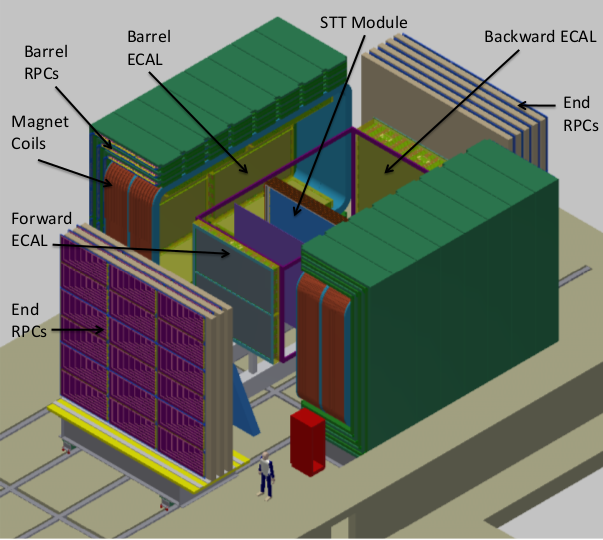
\includegraphics[width=0.63\textwidth, keepaspectratio=true]{figs/nearDetector.png}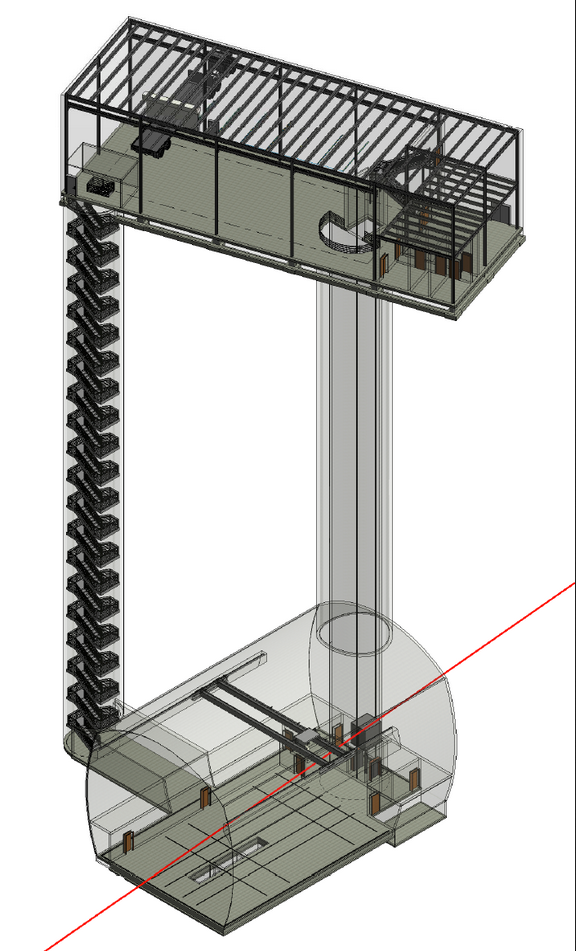
\includegraphics[width=0.35\textwidth, keepaspectratio=true]{figs/nearDetector_project.png}
\end{figure}

The ND would be located few hundred meters downstream the neutrino beam, and the neutrino beam would be much denser at this point than after traveling 1300 km to the FD, that is why the ND doesn't have to be as large as the FD. Also the ND aims on measuring neutrino fluxes with much higher precision than the FD to keep systematic uncertainty of the measurements at the FD smaller than expected statistical error for data collected during the whole expected time of operation.\\  

Because of different physics goals, the scheme of the ND (shown at the Fig. \ref{fig:nearDetector}) is also very different from the one of the FD. The detector will consist of central Straw-Tube Tracker (STT) modules, electromagnetic calorimeter (ECAL), magnet coils of 0.4T and muon identification system consisting of Resistive Plate Chamber (RPC) modules. The neutrinos would come from the bottom left corner of the picture, to the End RPCs. Different sorts of neutrino targets will be built into the tracker, in between the Straw-Tubes. The detector will be placed 60 meters underground.




